%-*- coding: UTF-8 -*-
% gougu.tex
% 勾股定理
\documentclass[UTF8]{ctexart}
\usepackage{graphicx}
\usepackage{float}
\usepackage{amsmath}
\usepackage{amsthm}
\usepackage{geometry}
\geometry{a6paper,centering,scale=0.8}
\usepackage[format=hang,font=small,textfont=it]{caption}
\usepackage[nottoc]{tocbibind}

\newenvironment{myquote}
{\begin{quote}\kaishu\zihao{-5}}
{\end{quote}}

\newcommand\degree{^\circ}

\title{\heiti 1.4 连通性}
\author{\kaishu 段鑫}
\date{\today}

\bibliographystyle{plain}

\newtheorem{thm}{定理}
\newtheorem{mydef}{定义}

\begin{document}
       
    \maketitle
     
    \begin{mydef}[连通]
    
    设图$G$是非空的(至少有一个顶点)。如果$G$中任意两个顶点有一条路连接,则称$G$是连通的(connected)。
    
    \end{mydef}
    
    \textbf{注:} 
    
    \begin{itemize}
    
      \item $K^1$是连通的。
      \item  $\forall u , v \in V(G),u \neq v , \exists$ 一条路  $P:u_{ 1 } u_{ 2 } u_{ 3 } ... u_{ k} u_{k+1}$  其中$u_{1}=u$,$u_{k+1}=v$ $u_{ i } \sim u_{i+1}  \quad i=1,2 ...k$。
      
     \end{itemize}
     \textbf{性质:} 设 $ G= ( V, E )$ 是 $n$ 个顶点 $ ( n \geq 2 )$ 连通图,
     则存在$ G $的一个序列$ v_{1}, v_{2},... v_{n}$, $ V_{G} =\lbrace v_{1}, v_{2},... v_{n} \rbrace$, $G\lbrack  v_{1}, v_{2},... v_{i}\rbrack $是连通的。 $ i=1,2 ...n$
    
    \textbf{证明:}数学归纳法
    
    $ i=1$ \qquad $G\lbrack  v_{1} \rbrack $只有一个顶点,是连通的。
    
    
    假设$ G\lbrack  v_{1}, v_{2},... v_{i} \rbrack $ 是连通的,其中$ i <|G| $
    存在  $ v \in V(G) \backslash \lbrace  v_{1}, v_{2},... v_{i} \rbrace $ 
    
    由于$ G $是连通的,存在从$ v $到$v_{1}$的一条路$P$,$P:v= u_{1}, u_{2},... u_{k+1}=v_{1}$
    
    取$ v_{i+1}$为$ P $ 在 $ G-G_{i} $中的最后一个顶点,则$ G\lbrack  v_{1}, v_{2},... v_{i},v_{i+1}\rbrack $是连通的。
    
    $\forall v_{s},v_{t} \in \lbrace  v_{1}, v_{2},... v_{i+1}\rbrace $
    
    \textbf{case 1:} $1\leq s,t\geq i$ 由于$G\lbrace  v_{1}, v_{2},... v_{i}\rbrace $连通,所以存在从$v_{s}$到$v_{t}$的一条路。
    
    \textbf{case 2:} $s=i+1$ or $t=i+1$ 不妨设 $s=i+1$ 因为在$G\lbrack v_{1}, v_{2},... v_{i+1}$中有从$v_{i+1}$ 到 $v_{1}$的一条路,
    在$ G\lbrack  v_{1}, v_{2},... v_{i} \rbrack$中有从$v_{i}$到$v_{t}$的一条路,所以$G\lbrack  v_{1}, v_{2},... v_{i+1}\rbrack$是连通的。
    
    由归纳原理可得性质成立。
    
    \begin{mydef}[连通分支]
    
    $G$的极大连通子图称为$G$的一个连通分支
    
    \end{mydef}
    
    对于$ G=( V(G),E(G) )$ ,$ H=( V(H),E(H) )$ 是它的一个连通分支。
    则有:$V(H)\subseteq V(G)$,$E(H)\subseteq E(G)$且$H$是连通的。
    
    若有$H_{1}$是图$G$的另一个子图,且有$V(H)\subseteq V(H_{1}) \subseteq V(G)$,$E(H)\subseteq  E(H_{1}) \subseteq E(G)$, $H_{1} \neq H$
    则$H_{1}$是不连通的。
    
    
    
    \begin{mydef}[A-B路]
    
    设$A,B \subseteq V$,称路$P=x_{0},x_{1}...x_{k}$为一条$A-B$路,如果$V(G) \cap A = x_{0}$,$V(G) \cap B = x_{k}$。当$ A= \lbrace a \rbrace $时,
    $A-B$ 路即为 $a-B$ 路。
    
    \end{mydef}
    
    
    \begin{mydef}[独立]
    
    两条(几条)路是独立(independent)如果这些路的内部顶点都不相同。(除非起点是终点)
    \end{mydef}
    
    $P=x_{0}x_{1}...x_{m}$,$Q=y_{0}y_{1}...y_{n}$,其中有 $ \lbrace x_{0}x_{1}...x_{m-1} \rbrace  \cap \lbrace  y_{0}y_{1}...y_{n-1} \rbrace  = \emptyset$,
    则$P$,$Q$这两条路独立。
    
    
    \begin{mydef}[H-路]
    
    如果$P$是非平凡的(至少有两个顶点),
    且$ V(G) \cap V(H) = \lbrace x_{0},x_{k}  \rbrace $,
    其中$ P = x_{0}x_{1}...x_{k}$,则$P$是一条$H-$路。
    
    \end{mydef}
    
    
    \begin{mydef}[分离]
    
    设$ A,B \subseteq V $,$ X \subseteq V \cup E $,
    使得每条 $A-B$ 路包含 $ X $中的一个元素,
    则称 $X $ 分离(seperate) $ G $中 $A$ 与$B$ 集合。
    
    \end{mydef}
    
    \textbf{注:}
    $A \cap B \subseteq  X$,且$ V \subseteq A \cap B  $,
    则 $V$是一条 $A-B$路。
    
    
     \begin{figure}[ht]
        \centering
        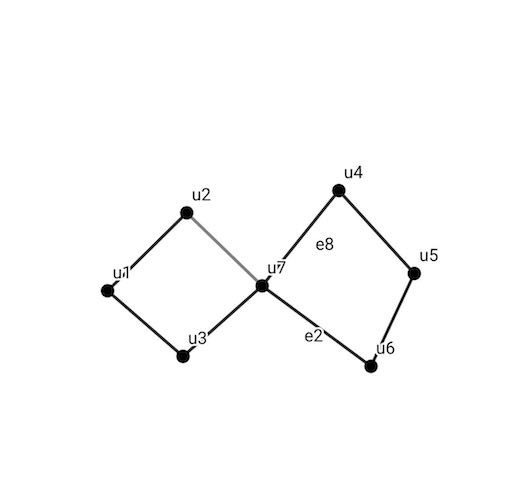
\includegraphics[scale=0.3]{tu1.png}
        \caption{$A= \lbrace u_{1},u_{2},u_{3} \rbrace, B= \lbrace u_{5},u_{6}\rbrace ,x_{1}= \lbrace u_{5},u_{6} \rbrace , x_{2} = \lbrace e_{8} \rbrace ,x_{3}= \lbrace e_{2}, e_{3} \rbrace, x_{4}= \lbrace u_{4} \rbrace , x_{5}= \lbrace u_{7} \rbrace $ 其中 $x_{1},x_{4},x_{5}$分离$A$与$B$集合,而$x_{2},x_{3}$没有分离$A$与$B$集合}
        \label{fig:tu1}
    \end{figure}
    
    
    \begin {mydef}[分离集]
    
    $X \subseteq V(G)$,如果$X$分离$G-X$中两个顶点,
    则称$X$分离$G$,且称$X$为$G$的一个分离集。
    
    \end{mydef}
    
    
    \begin{mydef}[割点]
    
    一个顶点分离$G$的一个连通分支,则称这个顶点为割点(cut vertex)。
   
    \end{mydef}
    
    \begin{mydef}[割边]
    一条边分离$G$中的一个连通分支,则称这条边为割边(egde cut)。
    \end{mydef}
    
    \begin{mydef}[k-连通]
    设$G$是一个图,若$|G|>k$, 并且对于$X \subseteq V(G), |X|<k $, $G-X$是连通的,则称$G$为k-连通的。
    \end{mydef}
    
    \textbf{注:}
    
    \begin{itemize}
    \item 对于$G$中任何两个顶点,能被小于$k$个顶点的集分离。
    \item 每个非空图是0-连通的。
    \item 1-连通图恰好是非平凡的连通图。
    \item $K^{1}$是0-连通的。(但是$K^{1}$是连通的)
    \end{itemize}
    
    
    \begin{mydef}[连通度]
    存在最大的非零整数$k$使得$G$是k-连通的,
    则称$G$的连通度(connectivity)为$k$,
    记作$\mathcal{K}(G)$。
    \end{mydef}
    
    \textbf{注:}
    \begin{itemize}
    
    \item $G$是 $k-$连通的,则G是k-1 -连通的。
    \item $\mathcal{K}(G)=0$  $\Longleftrightarrow$ $G=K^{1}$或者G是不连通的。
    \item $\mathcal{K}(G)=1$   $\Longleftrightarrow$ G是至少两个顶点的连通图,且有割点。
    \item $\mathcal{K}(K^{n})=n-1, n\geq 1$
    \item  $G \neq K^{n}, n\geq 2$ 则有$\mathcal{K}( G )= \leq n-2$
    
    \end{itemize}
    
     \begin{mydef}[$\mathit{l}$-边连通]
     $|G|>1$,对于$\forall F \subseteq E, |F| < \mathit{l} $,$G-F$是连通的,
     则称G是$ \mathit{l}$-边连通的。
     \end{mydef}
     
     \begin{mydef}[边连通度]
     存在最大非负整数$ \mathit{l} $使得G是$ \mathit{l} $-连通的,
     则称G的边连通度(edge connectivity)为 $\lambda(G)= \mathit{l}$。
     
    \end{mydef}
    
    \begin{thm}
    设G是至少有两个顶点的简单图,
    则有:
    $ \mathcal{K}(G)  \leq \lambda(G)  \leq \delta(G)$
    \end{thm}
    
    \textbf{证明:}
    
    
    \tableofcontents
    \section{勾股定理在古代}\label{sec:diyijie}
    西方称勾股定理为毕达哥拉斯定理,将勾股定理的发现归功于公元前 6 世纪的
    毕达哥拉斯学派 \cite{Kline}。该学派得到了一个法则,可以求出可排成直角
    三角形三边的三元数组。毕达哥拉斯学派没有书面著作,该定理的严格表述和证
    明则见于欧几里德\footnote{欧几里得,约公元前 330--275 年。}《几何原本》
    的命题 47:“直角三角形斜边上的正方形等于两直角边上的两个正方形之和。 ” 
    证明是用面积做的。
    
    我国《周髀算经》载商高(约公元前 12 世纪)答周公问:
    \begin{myquote}
        勾广三,股修四,径隅五。
    \end{myquote}
    又载陈子(约公元前 7--6 世纪)答荣方问:
    \begin{myquote}
        若求邪至日者,以日下为勾,日高为股,勾股各自乘,并而开方除之,得邪至日。
    \end{myquote}
    都较古希腊更早。后者已经明确道出勾股定理的一般形式。图\ref{fig:xiantu}是
    我国古代对勾股定理的一种证明 \cite{quanjing}。
   
    \section{勾股定理的近代形式}
    勾股定理可以用现代语言表述如下:
    \begin{thm}[勾股定理]
        直角三角形斜边的平方等于两腰的平方和。
    \end{thm}

    可以用符号语言表述为:设直角三角形$ABC$,其中$\angle C = 90\degree$,则有
    \begin{equation}\label{eq:gougu}
    AB^2 = BC^2 + AC^2.
    \end{equation}
    满足式\eqref{eq:gougu}的整数称为\emph{勾股数}。第\ref{sec:diyijie}节所说
    毕达哥拉斯学派得到的三元数组就是勾股数。下表列出一些较小的勾股数:
    \begin{table}[H]
        \begin{tabular}{|rrr|}
            \hline
            直角边 $a$ & 直角边 $b$ & 斜边 $c$ \\
            \hline
            3 & 4 & 5 \\
            5 & 12 & 13 \\
            \hline
        \end{tabular}%
        \qquad
        ($a^2 + b^2 = c^2$)
    \end{table}
    \nocite{Shiye}
    \bibliography{math}
\end{document}
